\lecture{6.3}{Manual Ensemble Construction}
\label{lec:6-3}

\subsection{Ensemble Prediction Functions}

An ensemble combines predictions from multiple fitted regressions. With two
candidate outcome regressions $\Qbar_{n,1}$ and $\Qbar_{n,2}$, a convex ensemble is
\[
\Qbar_{n,\omega}(a,w)
=
\omega \Qbar_{n,1}(a,w)+(1-\omega)\Qbar_{n,2}(a,w),
\qquad 0\le \omega\le 1.
\]
The weight $\omega$ controls how much the ensemble uses the first candidate. If
$\omega=1$, the ensemble is $\Qbar_{n,1}$. If $\omega=0$, the ensemble is
$\Qbar_{n,2}$.

\subsection{Weighted Averages of Candidate Predictions}

The following function takes two fitted \texttt{glm} objects, obtains predictions from
each, and returns their weighted average:

\begin{implementationbox}
\begin{lstlisting}[language=R]
ensemble_predict <- function(Q1_fit, Q2_fit, newdata,
                             Q1_weight, Q2_weight = 1 - Q1_weight) {
  stopifnot(abs(1 - Q1_weight - Q2_weight) < 1e-5)

  Q1n <- predict(Q1_fit, newdata = newdata)
  Q2n <- predict(Q2_fit, newdata = newdata)

  ensemble_prediction <- Q1_weight * Q1n + Q2_weight * Q2n
  as.numeric(ensemble_prediction)
}
\end{lstlisting}
\end{implementationbox}

For one new observation, this function computes
\[
\omega \hat y_1+(1-\omega)\hat y_2.
\]
For many observations, it computes the same formula row by row.

\subsection{Weight Grids}

With two candidates, a simple way to search over possible ensembles is to create a
grid of weights:

\begin{implementationbox}
\begin{lstlisting}[language=R]
weight_sequence <- seq(from = 0, to = 1, length.out = 500)
\end{lstlisting}
\end{implementationbox}

Each value in \texttt{weight\_sequence} defines a different candidate ensemble.
The grid is only an approximation to the continuum $[0,1]$, but it is sufficient for
illustrating the idea. With many candidates, the weight vector lies in a higher
dimensional simplex, and numerical optimization methods are used instead of a simple
grid.

\begin{figure}[H]
\centering
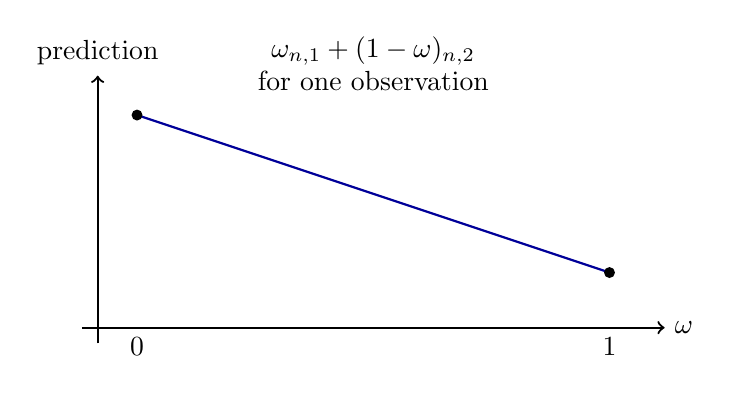
\begin{tikzpicture}[
  axis/.style={->, thick},
  pt/.style={circle, fill=black, inner sep=1.4pt}
]
\draw[axis] (-.2,0) -- (7.2,0) node[right] {$\omega$};
\draw[axis] (0,-.2) -- (0,3.2) node[above] {prediction};
\draw[thick, blue!60!black] (0.5,2.7) -- (6.5,.7);
\node[pt] at (.5,2.7) {};
\node[pt] at (6.5,.7) {};
\node[below] at (.5,0) {$0$};
\node[below] at (6.5,0) {$1$};
\node[align=center] at (3.5,3.35) {$\omega \Qbar_{n,1}+(1-\omega)\Qbar_{n,2}$\\for one observation};
\end{tikzpicture}
\caption{With two learners, ensemble predictions vary linearly with the weight.}
\label{fig:ch6-weight-path}
\end{figure}

\subsection{Cross-Validated Risk Across Weights}

For each weight, compute out-of-fold ensemble predictions and evaluate mean
squared-error loss. For a fixed $\omega$, the two-fold estimate is
\[
R_{CV,n}(\omega)
=
\frac{1}{2}
\left[
\frac{1}{n_1}\sum_{i\in \mathcal V_1}
\{Y_i-\Qbar_{n,\omega,2}(A_i,W_i)\}^2
+
\frac{1}{n_2}\sum_{i\in \mathcal V_2}
\{Y_i-\Qbar_{n,\omega,1}(A_i,W_i)\}^2
\right],
\]
where $\Qbar_{n,\omega,2}$ is the ensemble built from models trained in split 2 and
validated in split 1, and $\Qbar_{n,\omega,1}$ is the analogous ensemble trained in
split 1 and validated in split 2.

\begin{implementationbox}
\begin{lstlisting}[language=R]
cv_risks <- rep(NA_real_, length(weight_sequence))

for (i in seq_along(weight_sequence)) {
  w <- weight_sequence[i]

  pred_split2 <- ensemble_predict(Q1_fit_split1, Q2_fit_split1,
                                  newdata = split2,
                                  Q1_weight = w)
  risk_split2 <- mean((split2$Y - pred_split2)^2)

  pred_split1 <- ensemble_predict(Q1_fit_split2, Q2_fit_split2,
                                  newdata = split1,
                                  Q1_weight = w)
  risk_split1 <- mean((split1$Y - pred_split1)^2)

  cv_risks[i] <- (risk_split1 + risk_split2) / 2
}
\end{lstlisting}
\end{implementationbox}

\subsection{Selecting Optimal Ensemble Weights}

The Super Learner weight is the value with the smallest cross-validated risk:
\[
\omega_{CV}=\argmin_{\omega\in[0,1]}R_{CV,n}(\omega).
\]
On a grid, this is computed by:

\begin{implementationbox}
\begin{lstlisting}[language=R]
min_idx <- which.min(cv_risks)
omega_hat <- weight_sequence[min_idx]
min_cv_risk <- cv_risks[min_idx]
\end{lstlisting}
\end{implementationbox}

After the weight is selected, the candidate regressions are typically refit on the full
dataset. The final ensemble prediction function is
\[
\Qbar_{n,SL}(a,w)
=
\omega_{CV}\Qbar_{n,1}^{\mathrm{full}}(a,w)
+
(1-\omega_{CV})\Qbar_{n,2}^{\mathrm{full}}(a,w).
\]

\begin{keyidea}
Manual ensemble construction has two layers of learning. First, each candidate
regression learns from training data. Second, the ensemble learns weights by comparing
out-of-fold predictions.
\end{keyidea}

\begin{estimationbox}
When there are more than two candidates, Super Learner chooses weights
$\omega_1,\ldots,\omega_K$ satisfying $\omega_k\ge 0$ and $\sum_k\omega_k=1$.
Specialized optimization routines find the cross-validated risk minimizer over this
simplex more efficiently than a grid search.
\end{estimationbox}
